% Corrected re-typesetting of the PDF supplied in articles.zip.
% See CORRECTIONS.md for transcription repairs and substantive editorial notes.
% Compile twice with: pdflatex -interaction=nonstopmode -halt-on-error scheinerman2000.tex
\documentclass[11pt,letterpaper]{article}
\usepackage[utf8]{inputenc}
\usepackage[T1]{fontenc}
\usepackage{lmodern}
\usepackage[margin=0.88in,headheight=15pt,headsep=18pt]{geometry}
\usepackage{amsmath,amssymb,mathtools}
\usepackage{microtype}
\usepackage{graphicx,booktabs,array,longtable}
\usepackage{enumitem}
\usepackage{listings}
\usepackage{xurl}
\usepackage[hidelinks,unicode,pdfencoding=auto]{hyperref}
\usepackage{fancyhdr}
\usepackage{needspace}
\usepackage{tikz}
\usetikzlibrary{arrows.meta,positioning}
\urlstyle{same}
\setlength{\emergencystretch}{2em}
\setlength{\parskip}{2pt}
\setlength{\parindent}{1.2em}
\linespread{1.025}
\allowdisplaybreaks[1]
\setlist{itemsep=3pt,topsep=6pt,parsep=1pt}
\lstset{basicstyle=\ttfamily\small,columns=fullflexible,keepspaces=true,
  breaklines=true,breakatwhitespace=true,showstringspaces=false,
  aboveskip=9pt,belowskip=9pt,xleftmargin=0.6em}
\newcommand{\editorialnote}[1]{\begin{quote}\small\noindent
  \textbf{Editorial note.} #1\end{quote}}
\newcommand{\transcriptionnote}{\par\smallskip\noindent{\footnotesize
  Corrected re-typesetting. Original numbering retained; pagination reset.
  Substantive editorial changes are identified in the accompanying correction log.}\par\medskip}
\newcommand{\R}{\mathbb{R}}
\newcommand{\Q}{\mathbb{Q}}
\newcommand{\Z}{\mathbb{Z}}
\DeclareMathOperator{\sgn}{sgn}
\DeclareMathOperator{\Gal}{Gal}
\DeclareUnicodeCharacter{27F8}{\ensuremath{\Longleftarrow}}
\DeclareUnicodeCharacter{27F9}{\ensuremath{\Longrightarrow}}
\DeclareUnicodeCharacter{21D2}{\ensuremath{\Rightarrow}}
\DeclareUnicodeCharacter{21D4}{\ensuremath{\Leftrightarrow}}
\DeclareUnicodeCharacter{25A1}{\ensuremath{\square}}
\DeclareUnicodeCharacter{2264}{\ensuremath{\leq}}
\DeclareUnicodeCharacter{2265}{\ensuremath{\geq}}
\DeclareUnicodeCharacter{2212}{\ensuremath{-}}
\DeclareUnicodeCharacter{00B1}{\ensuremath{\pm}}
\DeclareUnicodeCharacter{00D7}{\ensuremath{\times}}
\pagestyle{fancy}
\fancyhf{}
\fancyhead[L]{\small\itshape Scheinerman: When Close Enough Is Close Enough}
\fancyhead[R]{\small\thepage}
\renewcommand{\headrulewidth}{0.3pt}
\fancypagestyle{plain}{\fancyhf{}\fancyfoot[C]{\small\thepage}\renewcommand{\headrulewidth}{0pt}}
\hypersetup{pdftitle={When Close Enough Is Close Enough},pdfauthor={Edward R. Scheinerman},pdfsubject={Corrected re-typesetting of the supplied article}}
\title{When Close Enough Is Close Enough}
\author{Edward R. Scheinerman}
\date{\small \emph{The American Mathematical Monthly} 107(6) (2000), 489--499.}

\begin{document}
\maketitle
\transcriptionnote

\section*{1. Prelude: An Interchange between an Algebra Teacher and Student}
A student was asked to demonstrate the following equation:

\[
\sqrt{2}+\sqrt{5-2 \sqrt{6}}=\sqrt{3} .
\]

\noindent\textbf{Teacher:} Please show me your solution to this problem.

\noindent\textbf{Student:} Sure. At first I was confused, but then I had a great idea. I just used my calculator. Both sides of the equation evaluate to 1.732050808 . So they're the same!

\noindent\textbf{Teacher:} Hmm. That's a good idea, but it doesn't really answer the question. You see, your calculator can display only 10 digits. It's possible that these two numbers agree to 10 decimal places, but aren't equal.

\noindent\textbf{Student:} Get out! I don't believe that two expressions that agree to that many digits could be different.

\noindent\textbf{Teacher:} Actually, they could. Let me give you an example. Do you have your calculator with you?

\noindent\textbf{Student:} Yes.

\noindent\textbf{Teacher:} Excellent. Please calculate

\[
\sqrt{75025}+\sqrt{121393}+\sqrt{196418}+\sqrt{317811} .
\]

\noindent\textbf{Student:} (after a brief pause) I get 1629.259889.

\noindent\textbf{Teacher:} Good. Now please calculate

\[
\sqrt{514229}+\sqrt{832040} .
\]

\noindent\textbf{Student:} (another brief pause) I get 1629.259889. Hey! That's the same as before. They're equal.

\noindent\textbf{Teacher:} Well, actually, they're not equal.

\noindent\textbf{Student:} How do you know?

\noindent\textbf{Teacher:} Let me show you on my computer. I have a program that will let us calculate these expressions with much greater accuracy than your calculator.

First I type

\begin{verbatim}
sqrt(75025) + sqrt(121393) + sqrt(196418) + sqrt(317811)
\end{verbatim}

and the computer responds: 1629.259888633142299848838800.

\noindent\textbf{Student:} Wow! That's 28 digits.

\noindent\textbf{Teacher:} It is nice. Now I type

\begin{verbatim}
sqrt(514229)+sqrt(832040)
\end{verbatim}

and the computer gives 1629.259888630189238404283301 . Look closely. Notice that the ninth digits after the decimal points are different. So you see, even though your calculator gives the same (approximate) value for the two expressions, that does not mean they are exactly equal.

Do you understand?

\noindent\textbf{Student:} You bet! You have a much better calculator than I have. May I try?

\noindent\textbf{Teacher:} Yes, but....

\noindent\textbf{Student:} Let's see. I type sqrt (2) + sqrt (5-2*sqrt (6) ) and hit return. I get \[1.732050807568877293527446341.\]

\noindent\textbf{Teacher:} Yes, but ... .

\noindent\textbf{Student:} And then I type sqrt (3) and-LOOK!-it gives me exactly the same answer: \[1.732050807568877293527446341.\] You see, they are equal.

Will we be allowed to use your computer on the test?

\noindent\textbf{Teacher:} Sigh!

\section*{2. Who Is Right?} This is not an article bemoaning the state of mathematics education. And I am sure that readers of this Monthly will have no trouble verifying that $\sqrt{2}+\sqrt{5-2 \sqrt{6}}$ and $\sqrt{3}$ are equal. Rather, my purpose is to defend the student.

The student's intuition is that if two algebraic expressions such as $\sqrt{2}+$ $\sqrt{5-2 \sqrt{6}}$ and $\sqrt{3}$ agree to 28 digits, then surely they are equal.

We transform the student's intuition by asking: When does $|\alpha-\beta|<\varepsilon$ imply $\alpha=\beta$ ? For example, if $\alpha$ and $\beta$ are integers, then if we know that $|\alpha-\beta|$ is (say) less than 0.9 , then we may conclude that $\alpha=\beta$.

Here is another example. Suppose $\alpha$ and $\beta$ are the two roots, counted with multiplicity, of some monic (leading coefficient equal to 1 ) quadratic polynomial with integer coefficients: $x^{2}+b x+c$. Then

\[
|\alpha-\beta|=\left|\sqrt{b^{2}-4 c}\right| .
\]

Since $b^{2}-4 c$ is an integer, we have either $\alpha=\beta$, or else $|\alpha-\beta| \geq 1$. So if we know that $|\alpha-\beta|<0.9$, we may conclude that $\alpha=\beta$.

The two sides of the equation $\sqrt{2}+\sqrt{5-2 \sqrt{6}}=\sqrt{3}$ are not integers. It is not a priori obvious that they are roots of a common, monic quadratic polynomial. However, one can show that $\sqrt{2}+\sqrt{5-2 \sqrt{6}}-\sqrt{3}$ is the root of some monic, integer polynomial; such roots are known as algebraic integers. Thus, one approach to making the student's intuition rigorous is to develop the theory of algebraic integers; see [16]. Instead, we present an equivalent theory based on eigenvalues of matrices; the proofs are sufficiently straightforward that they can be presented in an undergraduate linear algebra class. This will enable us to answer the question: When is close enough, close enough?

\section*{3. Eigenvalues Of Integer Matrices} Let $n$ and $b$ be positive integers. Let $M(n, b)$ denote the set of all $n \times n$ matrices whose entries are integers bounded in absolute value by $b$. That is, if $A \in M(n, b)$, then $A$ is $n \times n, a_{i j} \in \mathbb{Z}$, and $\left|a_{i j}\right| \leq b$. Let $\Lambda(n, b)$ denote the set of all eigenvalues of matrices in $M(n, b)$. Note that $\Lambda(n, b)$ is a finite set of complex numbers, and therefore we can bound the absolute values of its nonzero members away from zero (see Theorem 4).

\noindent\textbf{Proposition 1.} Let $A \in M(n, b)$. Then $\operatorname{det}(\lambda I-A)$ is a monic, integer polynomial.

(By integer polynomial we mean a polynomial whose coefficients are integers.)

\noindent\textit{Proof.} Use induction and the cofactor expansion formula. \(\square\)

\noindent\textbf{Proposition 2.} Let $\alpha$ be a complex number. Then $\alpha$ is an algebraic integer if and only if $\alpha \in \Lambda(n, b)$ for some positive integers $n, b$.

\noindent\textit{Proof.} If $\alpha$ is an algebraic integer, then it is the root of some monic, integer polynomial $p(x)$. Then $\alpha$ is an eigenvalue of the companion matrix of $p$, and so $\alpha \in \Lambda(n, b)$ for some $n, b$.

The converse follows from Proposition 1. \(\square\)

\noindent\textbf{Proposition 3.} Suppose $\alpha \in \Lambda(n, b)$. Then $|\alpha| \leq n b$.

\noindent\textit{Proof.} Suppose $\alpha$ is an eigenvalue of $A \in M(n, b)$ with corresponding eigenvector $\mathbf v$. Without loss of generality, we may assume that $\mathbf{v}$ is a unit vector, i.e., $\mathbf v^*\mathbf v=1$. Since $\mathbf v^*A\mathbf v=\mathbf v^*(\alpha\mathbf v)=\alpha$, we have

\[
\begin{aligned}
|\alpha| & =|\mathbf v^*A\mathbf v|=\left|\sum_{i} \sum_{j} \overline{v_i}\,a_{ij}v_j\right| \\
& \leq b \sum_{i} \sum_{j}\left|v_{i} v_{j}\right|=b \sum_{i}\left|v_{i}\right| \sum_{j}\left|v_{j}\right|=b\|\mathbf{v}\|_{1}^{2} .
\end{aligned}
\]

Here $\mathbf v^*$ denotes conjugate transpose. Since $\|\mathbf{v}\|_{1} \leq \sqrt{n}\|\mathbf{v}\|_{2}$ (see [8, problem 3, p. 278]) we have $|\alpha|\leq nb$. \(\square\)

The bound is best possible: Let $A$ be an $n \times n$ matrix all of whose entries are $b$. Let $\mathbf1$ be the vector of all 1s. Then $A \mathbf{1}=n b \mathbf{1}$.

\noindent\textbf{Theorem 4.} Suppose $A \in M(n, b)$ and $\alpha$ is a nonzero eigenvalue of $A$. Then $|\alpha| \geq(n b)^{1-n}$.

\noindent\textit{Proof.} Suppose the nonzero eigenvalues of $A$, counted with algebraic multiplicity, are $\alpha, \lambda_{2}, \ldots, \lambda_{t}$. The last nonzero coefficient of the characteristic polynomial of $A$ is $\pm \alpha \lambda_{2} \cdots \lambda_{t}$. By Proposition 1, this is an integer, hence $\left|\alpha \lambda_{2} \cdots \lambda_{t}\right| \geq 1$ and so

\[
|\alpha| \geq \frac{1}{\left|\lambda_{2} \cdots \lambda_{t}\right|} \geq(n b)^{1-t} \geq(n b)^{1-n} .
\] \(\square\)

\noindent\textbf{Theorem 4.} is known as a root separation theorem; see [2], [3], or [14]. It enables us to answer the question: When is close enough, close enough? Suppose we are given an algebraic expression, such as $\alpha=\sqrt{2}+\sqrt{5-2 \sqrt{6}}-\sqrt{3}$. We need to find integers $n$ and $b$ such that $\alpha \in \Lambda(n, b)$. Then we calculate a certified numerical enclosure of $\alpha$ narrow enough to show that $|\alpha|<(n b)^{1-n}$. From this, it follows that $\alpha=0$.

The issue, then, is: Given an algebraic expression $\alpha$, how do we find positive integers $n$ and $b$ such that $\alpha \in \Lambda(n, b)$ ? The next result gives us tools to find $n$ and $b$.

\noindent\textbf{Theorem 5.} Let $n, n_{1}, n_{2}, b, b_{1}, b_{2}$ be positive integers.

\begin{itemize}
  \item[] [1] If $\alpha$ is a root of a monic, integer polynomial of degree $n$ whose coefficients have absolute value no larger than $b$, then $\alpha \in \Lambda(n, b)$.
  \item[] [2] If $n_{1} \leq n_{2}$ and $b_{1} \leq b_{2}$, then $\Lambda\left(n_{1}, b_{1}\right) \subseteq \Lambda\left(n_{2}, b_{2}\right)$.
  \item[] [3] If $\alpha \in \Lambda(n, b)$, then $-\alpha$ and $\bar{\alpha} \in \Lambda(n, b)$.
  \item[] [4] If $k$ is an integer, then $k\in\Lambda(1,\max\{1,|k|\})$.
  \item[] [5] If $\alpha \in \Lambda\left(n_{1}, b_{1}\right)$ and $\beta \in \Lambda\left(n_{2}, b_{2}\right)$, then $\alpha \beta \in \Lambda\left(n_{1} n_{2}, b_{1} b_{2}\right)$.
  \item[] [6] If $\alpha \in \Lambda\left(n_{1}, b_{1}\right)$ and $\beta \in \Lambda\left(n_{2}, b_{2}\right)$, then $\alpha+\beta \in \Lambda\left(n_{1} n_{2}, b_{1}+b_{2}\right)$.
  \item[] [7] If $k$ is a positive integer and $\beta^{k} \in \Lambda(n, b)$, then $\beta \in \Lambda(n k, b)$.
\end{itemize}

We illustrate the use of Theorem 5 by solving the following type of problem: Given an algebraic expression $\alpha$, determine integers $n$ and $b$ such that $\alpha \in$ $\Lambda(n, b)$.

Consider the expression:

\[
\alpha=\sqrt{7} \times \sqrt[3]{5-\sqrt{2}} .
\]

The atoms of this expression are the integers 2, 5, and 7. By part 4, we have

\[
2 \in \Lambda(1,2), \quad 5 \in \Lambda(1,5), \quad \text { and } \quad 7 \in \Lambda(1,7) .
\]

Next we classify $\sqrt{2}$ and $\sqrt{7}$; by part 7, we have

\[
\begin{aligned}
& 2 \in \Lambda(1,2) \Rightarrow \sqrt{2} \in \Lambda(2,2) \\
& 7 \in \Lambda(1,7) \Rightarrow \sqrt{7} \in \Lambda(2,7) .
\end{aligned}
\]

The classification of $5-\sqrt{2}$ follows from parts 3 and 6:

\[
\left.\begin{array}{rl}
5 & \in \Lambda(1,5) \\
\sqrt{2} \in \Lambda(2,2) \Rightarrow-\sqrt{2} & \in \Lambda(2,2)
\end{array}\right\} \Rightarrow 5+(-\sqrt{2}) \in \Lambda(1 \cdot 2,5+2)=\Lambda(2,7) .
\]

To classify the cube root of $5-\sqrt{2}$ we use part 7:

\[
5-\sqrt{2} \in \Lambda(2,7) \Rightarrow \sqrt[3]{5-\sqrt{2}} \in \Lambda(2 \cdot 3,7)=\Lambda(6,7) .
\]

Finally, part 5 gives us the final classification:

\[
\left.\begin{array}{r}
\sqrt{7} \in \Lambda(2,7) \\
\sqrt[3]{5-\sqrt{2}} \in \Lambda(6,7)
\end{array}\right\} \Rightarrow \alpha=\sqrt{7} \times \sqrt[3]{5-\sqrt{2}} \in \Lambda(2 \cdot 6,7 \cdot 7)=\Lambda(12,49) .
\]

These calculations are illustrated in Figure 1.

\begin{figure}[htbp]
\centering
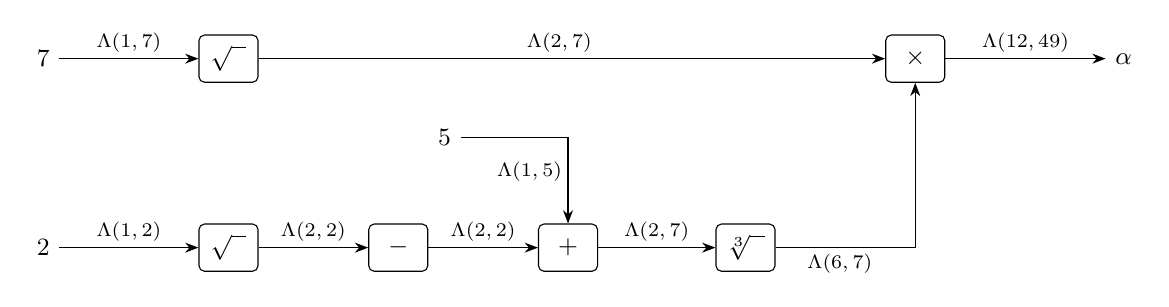
\begin{tikzpicture}[x=0.98cm,y=1cm,>=Stealth,
 op/.style={draw,rounded corners=2pt,minimum width=0.75cm,minimum height=0.6cm},
 every node/.style={font=\small},lab/.style={font=\scriptsize,fill=white,inner sep=2pt}]
\node (seven) at (0,1.7) {$7$};
\node[op] (sqrt7) at (2.4,1.7) {$\sqrt{\phantom{x}}$};
\node (two) at (0,-0.7) {$2$};
\node[op] (sqrt2) at (2.4,-0.7) {$\sqrt{\phantom{x}}$};
\node[op] (neg) at (4.6,-0.7) {$-$};
\node (five) at (5.2,0.7) {$5$};
\node[op] (plus) at (6.8,-0.7) {$+$};
\node[op] (cube) at (9.1,-0.7) {$\sqrt[3]{\phantom{x}}$};
\node[op] (mult) at (11.3,1.7) {$\times$};
\node (out) at (14,1.7) {$\alpha$};
\draw[->] (seven)--node[lab,above] {$\Lambda(1,7)$}(sqrt7);
\draw[->] (sqrt7)--node[lab,above,pos=.48] {$\Lambda(2,7)$}(mult);
\draw[->] (two)--node[lab,above] {$\Lambda(1,2)$}(sqrt2);
\draw[->] (sqrt2)--node[lab,above] {$\Lambda(2,2)$}(neg);
\draw[->] (neg)--node[lab,above] {$\Lambda(2,2)$}(plus);
\draw[->] (five) -| node[lab,pos=.7,left] {$\Lambda(1,5)$}(plus);
\draw[->] (plus)--node[lab,above] {$\Lambda(2,7)$}(cube);
\draw[->] (cube) -| node[lab,pos=.23,below] {$\Lambda(6,7)$}(mult);
\draw[->] (mult)--node[lab,above] {$\Lambda(12,49)$}(out);
\end{tikzpicture}
\caption{Using Theorem 5 to classify an algebraic expression.}
\end{figure}

The proof of Theorem 5 is given in the next section. However, we encourage the reader to be impatient and to proceed directly to Section 5. Return to the proof on your second reading.

\section*{4. Proof of Theorem 5}
\noindent\textit{Proof.} For part 1, see the proof of Proposition 2.

For part 2, suppose $\alpha$ is an eigenvalue of $A \in M\left(n_{1}, b_{1}\right)$. Let $B$ be the $n_{2} \times n_{2}$ matrix $\left[\begin{array}{cc}A & 0 \\ 0 & 0\end{array}\right] \in M\left(n_{2}, b_{2}\right)$. Since $\alpha$ is also an eigenvalue of $B$, it follows that $\alpha \in \Lambda\left(n_{2}, b_{2}\right)$.

For part 3, suppose $\alpha$ is an eigenvalue of $A \in M(n, b)$. Then $\bar{\alpha}$ is also an eigenvalue of $A$ and $-\alpha$ is an eigenvalue of $-A$. Hence $-\alpha, \bar{\alpha} \in \Lambda(n, b)$.

For part 4, note that $k$ is the eigenvalue of the matrix $[k]$.


For parts 5 and 6 we use the Kronecker (tensor) product of matrices [6]. Suppose $A$ is a $p \times q$ matrix and $B$ is an $r \times s$ matrix. The Kronecker product of $A$ and $B$ is the $p r \times q s$ matrix

\[
A \otimes B=\left[\begin{array}{cccc}
a_{11} B & a_{12} B & \cdots & a_{1 q} B \\
a_{21} B & a_{22} B & \cdots & a_{2 q} B \\
\vdots & \vdots & \ddots & \vdots \\
a_{p 1} B & a_{p 2} B & \cdots & a_{p q} B
\end{array}\right]
\]

One checks that if $\mathbf v$ is a $q$-vector and $\mathbf w$ is an $s$-vector, then

\[
(A \otimes B)(\mathbf{v} \otimes \mathbf{w})=(A \mathbf{v}) \otimes(B \mathbf{w}) .
\]

Now suppose $\alpha$ is an eigenvalue of $A \in M\left(n_{1}, b_{1}\right)$ corresponding to an eigenvector $\mathbf v$. Likewise, suppose $\beta$ is an eigenvalue of $B \in M\left(n_{2}, b_{2}\right)$ corresponding to an eigenvector $\mathbf{w}$. Then $A \otimes B \in M\left(n_{1} n_{2}, b_{1} b_{2}\right)$ and

\[
(A \otimes B)(\mathbf{v} \otimes \mathbf{w})=(A \mathbf{v}) \otimes(B \mathbf{w})=(\alpha \mathbf{v}) \otimes(\beta \mathbf{w})=(\alpha \beta)(\mathbf{v} \otimes \mathbf{w}),
\]

and so $\alpha \beta$ is an eigenvalue of $A \otimes B$ and hence is in $\Lambda\left(n_{1} n_{2}, b_{1} b_{2}\right)$.\\
Next, let $C=A \otimes I_{n_{2}}+I_{n_{1}} \otimes B$, so $C \in M\left(n_{1} n_{2}, b_{1}+b_{2}\right)$. Observe that

\[
\begin{aligned}
C(\mathbf{v} \otimes \mathbf{w}) & =\left(A \otimes I_{n_{2}}\right)(\mathbf{v} \otimes \mathbf{w})+\left(I_{n_{1}} \otimes B\right)(\mathbf{v} \otimes \mathbf{w}) \\
& =(A \mathbf{v} \otimes \mathbf{w})+(\mathbf{v} \otimes B \mathbf{w}) \\
& =\alpha(\mathbf{v} \otimes \mathbf{w})+\beta(\mathbf{v} \otimes \mathbf{w})=(\alpha+\beta)(\mathbf{v} \otimes \mathbf{w}) .
\end{aligned}
\]

Hence $\alpha+\beta$ is an eigenvalue of $C$ and therefore is in $\Lambda\left(n_{1} n_{2}, b_{1}+b_{2}\right)$.\\
Finally, for part 7, the case $k=1$ is immediate. For $k\geq2$, let $\alpha \in \Lambda(n, b)$. Suppose $\beta$ is a $k^{\text {th }}$ root of $\alpha$, i.e., $\beta^{k}=\alpha$. Let $A \in M(n, b)$ be a matrix for which $\alpha$ is an eigenvalue and let $\mathbf{v}$ be a corresponding eigenvector.

Let $B$ be the $n k \times n k$ matrix with block structure

\[
B=\left[\begin{array}{cccccc}
0 & I & 0 & 0 & \cdots & 0 \\
0 & 0 & I & 0 & \cdots & 0 \\
0 & 0 & 0 & I & \cdots & 0 \\
\vdots & \vdots & \vdots & \vdots & \ddots & \vdots \\
0 & 0 & 0 & 0 & \cdots & I \\
A & 0 & 0 & 0 & \cdots & 0
\end{array}\right] .
\]

Note that $B \in M(n k, b)$.

Define the vector $\mathbf{w}$ to be

\[
\mathbf{w}=\left[\begin{array}{c}
\mathbf{v} \\
\beta \mathbf{v} \\
\beta^{2} \mathbf{v} \\
\vdots \\
\beta^{k-2} \mathbf{v} \\
\beta^{k-1} \mathbf{v}
\end{array}\right] .
\]

We calculate

\[
B \mathbf{w}=\left[\begin{array}{c}
\beta \mathbf{v} \\
\beta^{2} \mathbf{v} \\
\beta^{3} \mathbf{v} \\
\vdots \\
\beta^{k-1} \mathbf{v} \\
A \mathbf{v}
\end{array}\right]=\left[\begin{array}{c}
\beta \mathbf{v} \\
\beta^{2} \mathbf{v} \\
\beta^{3} \mathbf{v} \\
\vdots \\
\beta^{k-1} \mathbf{v} \\
\alpha \mathbf{v}
\end{array}\right]=\left[\begin{array}{c}
\beta \mathbf{v} \\
\beta^{2} \mathbf{v} \\
\beta^{3} \mathbf{v} \\
\vdots \\
\beta^{k-1} \mathbf{v} \\
\beta^{k} \mathbf{v}
\end{array}\right]=\beta \mathbf{w}
\]

and therefore $\beta$ is an eigenvalue of $B$. Thus $\beta \in \Lambda(n k, b)$. \(\square\)

\section*{5. Proof of an Identity}
\editorialnote{A displayed zero, or agreement of rounded decimal strings, is not by itself an error bound. In this section, ``calculate to sufficient precision'' means obtain a proven enclosure, using outward-rounded interval arithmetic or an equivalent rigorous error estimate, whose entire absolute-value range is below the separation threshold. The accompanying \texttt{verify\_intervals.py} uses integer fixed-point interval endpoints, exact floor/ceiling operations, integer root bounds, and explicit Taylor remainder bounds. It independently certifies all four identity residuals below at absolute error less than $10^{-170}$. The historical \texttt{Recognize} command is retained as a conjecture generator, not as an identity proof.} Theorems 4 and 5 give us a technique to prove identities. We begin by re-expressing the identity in the form $\alpha \stackrel{?}{=} 0$. We use Theorem 5 to find $n$ and $b$ for which $\alpha \in \Lambda(n, b)$. By Theorem 4, if $\alpha \neq 0$, then $|\alpha| \geq(n b)^{1-n}$. We then calculate a certified numerical enclosure of $\alpha$ to show $|\alpha|<$ $(n b)^{1-n}$, and we conclude $\alpha=0$.

We illustrate this technique by proving the student's identity:

\[
\sqrt{2}+\sqrt{5-2 \sqrt{6}}=\sqrt{3} .
\]

The first step is to apply Theorem 5 to find integers $n$ and $b$ so that $\alpha=\sqrt{2}$ $+\sqrt{5-2 \sqrt{6}}-\sqrt{3} \in \Lambda(n, b)$.

Since $2 \in \Lambda(1,2)$ (part 4) we have $\sqrt{2} \in \Lambda(2,2)$ (part 7).\\
Likewise, $\sqrt{3} \in \Lambda(2,3)$, and so $-\sqrt{3} \in \Lambda(2,3)$ (part 3).\\
Since $\sqrt{6} \in \Lambda(2,6)$ and $-2 \in \Lambda(1,2)$, we have $-2 \sqrt{6} \in \Lambda(2,12)$ (part 5). Since $5 \in \Lambda(1,5)$, we have $5-2 \sqrt{6} \in \Lambda(2,17)$ (part 6). Hence $\sqrt{5-2 \sqrt{6}} \in \Lambda(4,17)$.

Finally, $\alpha=\sqrt{2}+\sqrt{5-2 \sqrt{6}}-\sqrt{3}$ is in $\Lambda(2 \cdot 4 \cdot 2,2+17+3)=\Lambda(16,22)$ (part 6).

Now we apply Theorem 4. If $\alpha \neq 0$ we would have

\[
|\alpha| \geq(16 \cdot 22)^{-15} \approx 6.3 \times 10^{-39} .
\]

However, a certified enclosure with $|\alpha|<10^{-44}$ suffices, so $\alpha=0$. The independent interval check accompanying this re-typesetting gives the stronger bound $|\alpha|<10^{-170}$.

To ease the computational burden, we want to find the smallest $n$ and $b$ for which $\alpha \in \Lambda(n, b)$. For example, consider the term $2 \sqrt{6}$. We showed that $2 \sqrt{6} \in \Lambda(2,12)$. Can we do better? Rewriting $2 \sqrt{6}$ as $\sqrt{24}$ doesn't help, because $24 \in \Lambda(1,24)$ and then part 7 gives $2 \sqrt{6}=\sqrt{24} \in \Lambda(2,24)$. However, it is easy to see that $\sqrt{24}$ is an eigenvalue of $\left[\begin{array}{ll}0 & 6 \\ 4 & 0\end{array}\right]$. Thus, $2 \sqrt{6} \in \Lambda(2,6)$.

In general, we have the following.\\
\noindent\textbf{Proposition 6.} If $a$ and $b$ are integers, then $\sqrt{a b} \in \Lambda(2,\max\{1,|a|,|b|\})$. \(\square\)

Using $2 \sqrt{6} \in \Lambda(2,6)$ improves our earlier analysis to $\alpha \in \Lambda(16,16)$ and so the separation bound is $(16 \cdot 16)^{-15} \approx 7.5 \times 10^{-37}$, a modest gain of two digits.

We can improve the bound a little more by recognizing $5-2 \sqrt{6}$ as a root of the quadratic equation $x^{2}-10 x+1=0$, giving $5-2 \sqrt{6} \in \Lambda(2,10)$, leading to $\alpha \in$ $\Lambda(16,15)$ and a separation bound of roughly $2 \times 10^{-36}$.

However, the recognition of $5-2 \sqrt{6}$ as a root of $x^{2}-10 x+1$ is far from automatic and such recognition may be difficult for more complicated expressions. Fortunately, this can be reduced to a calculation.

Given a numeric approximation of an expression, such as $5-2 \sqrt{6}$, symbolic mathematics software can find a low-degree polynomial with a root (nearly) equal to the given expression.

For example, in Mathematica, we can calculate as follows:

\begin{verbatim}
Needs["NumberTheory`Recognize`"]
a=5-2Sqrt[6];
Recognize[N[a],2,x]
        2
    1-10 x+x
\end{verbatim}

The first line loads the Recognize package. The second line defines a to be $5-2 \sqrt{6}$. The third line asks Mathematica to find a degree- 2 polynomial in x of which (a numerical approximation of) a is a root.

The recognition of $\alpha$ as a root of some polynomial is a computation. Can we also reduce the proof that $\alpha$ is the root of some polynomial to a computation?

For example, if we let $\alpha=\sqrt[3]{5 \sqrt{13}-18}$, Mathematica asserts that $\alpha$ is a root of $x^{2}+3 x-1=0$. We might try to verify this by expanding $\alpha^{2}+3 \alpha-1$ and checking to see if we get zero. However, that leads to the messy expression

\[
(5 \sqrt{13}-18)^{2 / 3}+3(5 \sqrt{13}-18)^{1 / 3}-1
\]

and I don't want to be bothered wrestling with that. I want to crunch those numbers, get something near zero, and be convinced.

One way to verify that $\alpha$ is a root of $p(x)=x^{2}+3 x-1$ is to apply the earlier method, i.e., find $n$ and $b$ so that $p(\alpha) \in \Lambda(n, b)$. Using $\alpha\in\Lambda(6,43)$ as below, the separate-expression rules give
\[
\alpha^2\in\Lambda(36,1849),\qquad 3\alpha\in\Lambda(6,129),
\]
and hence $p(\alpha)\in\Lambda(216,1979)$. Thus this direct application of the separation bound requires

\[
|p(\alpha)|<(216\cdot1979)^{-215}\approx2.27\times10^{-1211} .
\]

And while computers can calculate to that level of accuracy, a looser bound is clearly desirable.

Using Theorem 5 and Proposition 6, we can place $\alpha=\sqrt[3]{5 \sqrt{13}-18} \in \Lambda(6,43)$. Therefore, there is an $A \in M(6,43)$ with eigenvalue $\alpha$. Note that $p(\alpha)$ is an eigenvalue of $B=p(A)$. We can bound the absolute value of the entries of $B$ as follows. Let $J$ be the $6 \times 6$ matrix of all 1 s . Then

\[
|B|=|p(A)| \leq\left|A^{2}\right|+3|A|+I \leq(43 J)^{2}+3(43 J)+I \leq(6\cdot43^2+3\cdot43+1)J=11224J .
\]

(For a matrix $X$ whose $i, j$-entry is $x_{i j}$, we write $|X|$ for the matrix whose $i, j$-entry is $\left|x_{i j}\right|$.)

Therefore $p(\alpha) \in \Lambda(6,11224)$. To prove that $p(\alpha)=0$ it is enough to show that

\[
|p(\alpha)|<(6 \cdot 11224)^{-5} \approx 7.22\times10^{-25} .
\]

A certified interval calculation verifies this (the accompanying check gives $|p(\alpha)|<10^{-170}$), and therefore $\alpha$ is a root of $x^{2}+3 x-1$. Since $\alpha \approx 0.3028$ and since the two roots of $x^{2}+3 x-1=0$ are $\frac{1}{2}(-3 \pm \sqrt{13})$ we have proved that

\[
\sqrt[3]{5 \sqrt{13}-18}=\frac{-3+\sqrt{13}}{2} .
\]

We return to the earlier student/teacher example: We want to show that $\alpha$ $=\sqrt{2}+\sqrt{5-2 \sqrt{6}}$ is a root of $p(x)=x^{2}-3=0$. By Theorem 5 and Proposition 6, we have $\alpha \in \Lambda(8,13)$, and so there is a matrix $A \in M(8,13)$ of which $\alpha$ is an eigenvalue. Hence, $p(\alpha)=\alpha^{2}-3$ is an eigenvalue of $B=p(A)$. We have

\[
|B|=|p(A)|=\left|A^{2}-3 I\right| \leq\left|(13 J)^{2}\right|+3 I=1352 J+3 I
\]

where $J$ is the $8 \times 8$ matrix of all ones. Thus $B \in M(8,1355)$. Writing $\beta=p(\alpha)$, by Theorem 4, if $\beta\ne0$ we would have

\[
|p(\alpha)|=|\beta| \geq(8 \cdot 1355)^{-7} \approx 5.7 \times 10^{-29} .
\]

However, a certified enclosure gives $|p(\alpha)|<10^{-30}$ (indeed $<10^{-170}$ in the accompanying check), and so we may conclude that $p(\alpha)=0$, and so $\sqrt{2}+\sqrt{5-2 \sqrt{6}}=\sqrt{3}$.

In general, suppose $\alpha \in \Lambda(n, b)$ and $p$ is a monic, integer polynomial of degree $d$ whose coefficients are bounded in absolute value by $c$. Then we can easily calculate a positive $\varepsilon_{n, b, d, c}$ so that

\[
|p(\alpha)|<\varepsilon_{n, b, d, c} \Rightarrow p(\alpha)=0 .
\]

\section*{6. A More Complicated Example} We have presented a simple method for proving algebraic identities formed from integers using the operations +, -, $\times$, and $\sqrt[k]{ }$. One applies the rules in Theorem 5 to find $n$ and $b$ with $\alpha \in \Lambda(n, b)$. Then we calculate a certified numerical enclosure of $\alpha$ to verify that $|\alpha|<(n b)^{1-n}$. Then Theorem 4 implies that $\alpha=0$.


Now for a harder example. We solve Problem \#10756 from the October 1999 issue of this Monthly. The problem asks us to prove:

\[
\cos \frac{\pi}{7}=\frac{1}{6}+\frac{\sqrt{7}}{6}\left[\cos \left(\frac{1}{3} \arccos \frac{1}{2 \sqrt{7}}\right)+\sqrt{3} \sin \left(\frac{1}{3} \arccos \frac{1}{2 \sqrt{7}}\right)\right] .
\]

From

\[
\cos (n \theta)+i \sin (n \theta)=(\cos \theta+i \sin \theta)^{n}=\sum_{k=0}^n\binom{n}{k}(\cos \theta)^{k}(i \sin \theta)^{n-k}
\]

and the identity $\cos ^{2} \theta+\sin ^{2} \theta=1$ we get the following identities:

\[
\cos 3 \theta=4 \cos ^{3} \theta-3 \cos \theta
\]

and

\[
\cos 7 \theta=64 \cos ^{7} \theta-112 \cos ^{5} \theta+56 \cos ^{3} \theta-7 \cos \theta .
\]

Substituting $\theta=\pi/7$ and $\alpha=2 \cos (\pi / 7)$ into the second identity gives

\[
-1=\frac{1}{2} \alpha^{7}-\frac{7}{2} \alpha^{5}+7 \alpha^{3}-\frac{7}{2} \alpha
\]

or equivalently

\[
0=\alpha^{7}-7 \alpha^{5}+14 \alpha^{3}-7 \alpha+2=\left(\alpha^{3}-\alpha^{2}-2 \alpha+1\right)^{2}(\alpha+2) .
\]

Clearly $\alpha \neq-2$, so $\alpha=2 \cos (\pi / 7) \in \Lambda(3,2)$.

Next we tackle the term

\[
\sqrt{7} \cos \left(\frac{1}{3} \arccos \frac{1}{2 \sqrt{7}}\right) .
\]

In $\cos 3 \theta=4 \cos ^{3} \theta-3 \cos \theta$ we take


\begin{equation*}
\theta=\frac{1}{3} \arccos \frac{1}{2 \sqrt{7}} \tag{1}\label{eq:1}
\end{equation*}


and let $\beta_{0}=\cos \theta$. Then we have

\[
\frac{1}{2 \sqrt{7}}=4 \beta_{0}^{3}-3 \beta_{0} .
\]

Taking $\beta=2 \sqrt{7} \beta_{0}$ this becomes $\beta^{3}-21 \beta-7=0$, so

\[
\beta=2 \sqrt{7} \cos \left(\frac{1}{3} \arccos \frac{1}{2 \sqrt{7}}\right) \in \Lambda(3,21) .
\]

Now we deal with the sine term. From $\sin 3 \theta=-4 \sin ^{3} \theta+3 \sin \theta$ with $\theta$ defined by (1) we have $\sin 3 \theta=\sqrt{27 / 28}$. Let $\gamma_{0}=\sin \theta$ and we have

\[
4 \gamma_{0}^{3}-3 \gamma_{0}+\sqrt{\frac{27}{28}}=0 .
\]

Let $\gamma=2 \sqrt{7} \cdot \sqrt{3} \gamma_{0}$ to rewrite this as $\gamma^{3}-63 \gamma+189=0$. Therefore, $\gamma=$ $2 \sqrt{7} \cdot \sqrt{3} \sin \theta \in \Lambda(3,189)$.

Recapping, we have

\[
\begin{gathered}
\alpha=2 \cos \frac{\pi}{7} \in \Lambda(3,2), \quad \beta=2 \sqrt{7} \cos \theta \in \Lambda(3,21), \quad \text { and } \\
\gamma=2 \sqrt{7} \cdot \sqrt{3} \sin \theta \in \Lambda(3,189)
\end{gathered}
\]

where $\theta$ is defined by (1).

We can reexpress the Monthly problem as

\[
\zeta=6 \alpha-2-\beta-\gamma \stackrel{?}{=} 0 .
\]

Since $6 \alpha \in \Lambda(3,12)$, we have

\[
\zeta \in \Lambda(3 \cdot 3 \cdot 3,12+2+21+189)=\Lambda(27,224) .
\]

Therefore, if $\zeta \neq 0$ we would have $|\zeta| \geq(27 \cdot 224)^{-26} \approx 4.77 \times 10^{-99}$, but a certified interval calculation gives $|\zeta|<10^{-100}$ (indeed $<10^{-170}$ in the accompanying check), and so $\zeta=0$.

\section*{7. Computer Science Applications} This "close enough" technique for proving algebraic identities is a fun application of algebraic integers via linear algebra. Surprisingly, this method finds direct application in computer science.

Computational geometers develop their algorithms using a model of computation known as "the real RAM". In this model, an arbitrary real number consumes a single unit of storage, and the primitive operations are exact real arithmetic and exact tests of equality and order.

Initially, when these algorithms were deployed on actual computers, the idealized real RAM was replaced by floating point arithmetic. The results were disappointing. Round-off errors resulted in program failure.

Consequently, computer scientists sought a way to handle real numbers on real computers. The basic geometric objects handled by computational geometers are points, lines/line segments, and circles/arcs. Hence, the arena of today's computational geometers is the same as that of the ancient Greeks, and the real numbers they encounter are all constructible: formed from integers using the basic operations $+$, $-$, $\times$, $\div$, and $\sqrt{\phantom{x}}$.

Computational geometry "kernels" are now being developed that hold real numbers as a data structure of nested radicals; see [4], [15], and [17]. Equality testing is done by numerically approximating the expressions to sufficiently many digits to guarantee the results.

The close-enough method for verifying identities can be computationally inefficient. The verification of a modestly complicated expression might require an enormous number of digits. For positive integers $a_i$, an expression of the form
$\sqrt{a_1}\pm\sqrt{a_2}\pm\cdots\pm\sqrt{a_t}$ is, by Theorem 5, in
$\Lambda(2^t,a_1+\cdots+a_t)$. A sufficient test for zero is therefore that its \emph{absolute value} be less than
\[
 \left(2^t\sum_{i=1}^t a_i\right)^{1-2^t}.
\]
This direct test can require exponentially many digits as a function of $t$.

Computational geometers are aware of this issue, and some have developed an approach to geometric algorithm design that studies the asymptotic running time of algorithms that are restricted to using primitives involving algebraic quantities whose polynomial is of bounded degree; see [12].

However, automatic verification of nested radical identities need not be so computationally intensive. For an alternate, algebraic approach, see the work of Landau in [9], [10], and [11].

\section*{8. Final Remarks} We have presented a technique for proving identities involving algebraic integers. We classify the quantities involved as members of the classes $\Lambda(n, b)$ and then calculate numerically to sufficiently high precision to conclude equality. The technique can be extended to more general algebraic numbers by judiciously clearing denominators.

The technique raises a final question: Does a computer-assisted, calculation proof of a radical identity truly constitute a rigorous proof? The issue we need to consider is: Can we trust the computer and the programs it runs? In light of the early Pentium floating point flaws, it seems prudent to question the accuracy of calculations performed by computers. The CPU-resident floating point operations are beyond the inspection of nearly all computer users. However, there are public domain, arbitrary precision software programs (such as pari [1] and the Gnu MP package [7]) whose source code is available for inspection. In principle, one could check these programs in the same manner that one checks proofs in mathematics. Has this been done?

ACKNOWLEDGMENTS. Many thanks to Susan Landau and Michael Goodrich for their help with the computer science background material. Thanks also to Lara Diamond and David Marchette for their comments on early drafts of this article.

\begin{thebibliography}{99}
\bibitem{ref1} C. Batut and K. Belabas and D. Bernardi and H. Cohen and M. Olivier, Pari-GP home page: \href{http://hasse.mathematik.tu-muenchen.de/ntsw/pari/Welcome}{http://hasse.mathematik.tu-muenchen.de/ntsw/pari/Welcome}.

\bibitem{ref2} B. Buchberger, G. E. Collins, and R. Loos, editors, Computer Algebra: Symbolic and Algebraic Computation, second edition, Springer-Verlag, Vienna, 1983.

\bibitem{ref3} C. Burnikel, R. Fleischer, K. Mehlhorn, and S. Schirra, A strong and easily computable separation bound for arithmetic expressions involving square roots, in Proceedings of the Eighth Annual ACM-SIAM Symposium on Discrete Algorithms, Society for Industrial and Applied Mathematics, Philadelphia, 1997, pp. 702-709.

\bibitem{ref4} C. Burnikel, R. Fleischer, K. Mehlhorn, and S. Schirra, Efficient exact geometric computation made easy, in Proceedings of the Fifteenth Annual Symposium on Computational Geometry, ACM Press, 1999, pp. 341-350.

\bibitem{ref5} Henri Cohen, A Course in Computational Algebraic Number Theory, 3rd corrected edition, Number 138 in Graduate Texts in Mathematics, Springer-Verlag, Berlin, 1996.

\bibitem{ref6} Shaun Fallat, Algebraic integers and tensor products of matrices, Crux Math, 22 (1996) 341-343.

\bibitem{ref7} GMP home page: \href{http://www.gnu.org/software/gmp/gmp.html}{http://www.gnu.org/software/gmp/gmp.html}.

\bibitem{ref8} Roger A. Horn and Charles R. Johnson, Matrix Analysis, Cambridge University Press, New York, 1985.

\bibitem{ref9} Susan Landau, A note on ``Zippel denesting'', J. Symbolic Comput. 13 (1992) 41--46.

\bibitem{ref10} Susan Landau, Simplification of nested radicals, SIAM J. Comput., 21 (1992) 85-110.

\bibitem{ref11} Susan Landau, How to tangle with a nested radical, Math Intelligencer, 16 (1994) no. 2, 49-55.

\bibitem{ref12} Giuseppe Liotta, Franco P. Preparata and Roberto Tamassia, Robust proximity queries: An illustration of degree-driven algorithm design, in Proceedings of the Thirteenth Annual Symposium on Computational Geometry, ACM Press, 1997, pp. 156-165.

\bibitem{ref13} László Lovász, An Algorithmic Theory of Numbers, Society for Industrial and Applied Mathematics, Philadelphia, 1986.

\bibitem{ref14} Maurice Mignotte, Mathematics for Computer Algebra, Springer-Verlag, New York, 1992.

\bibitem{ref15} Michael Seel, LEDA home page: \url{http://www.mpi-sb.mpg.de/LEDA/}.

\bibitem{ref16} Ian Stewart and David Tall, Algebraic Number Theory, Chapman and Hall, New York, 1979.

\bibitem{ref17} Chee Yap, Exact geometric computation page: \href{http://cs.nyu.edu/exact/}{http://cs.nyu.edu/exact/}.

\bibitem{ref18} Chee Yap, Fundamental Problems in Algorithmic Algebra, Oxford University Press, Oxford, 2000.
\end{thebibliography}


\subsection*{Original Author Biography (2000)}
Edward R. Scheinerman is a professor in the Mathematical Sciences Department at the Johns Hopkins University. He was an undergraduate mathematics major at Brown, and received his Ph.D. in mathematics from Princeton. His research interests are in discrete mathematics. During academic year 1999-2000, he is an "internal visitor" to the Department of Mechanical Engineering at Hopkins.

Department of Mathematical Sciences, The Johns Hopkins University, Baltimore, MD 21218

\href{mailto:ers@jhu.edu}{ers@jhu.edu}

\end{document}
